% !TeX spellcheck = en_US
% !TeX root = ../build/road-to-scalability.tex
% !TeX TXS-program:compile = txs:///xelatex/[--shell-escape]



%%%%%%%%%%%%%%%%%%%%%%%%%%%%%%%%%%%%%%%%%%%%%%%%%%%%%%%%%%%%%%%%%%%%%%%%%%
\section{Introduction}

In this brief topic, we'll focus on \textbf{reorganizations}. The \textbf{synchronizer} is responsible for managing this process, alongside other tasks. We'll explore both L2 and L1 reorganizations, as well as touch a little bit upon the role of the synchronizer.


\section{L2 Reorganizations}

First, we show a situation in which there is a reorganization of L2 batches:

Consider that there is a certain sequencer (let's call it sequencer A) that has closed the batch 724. So, the batch $\mathtt{724^A}$ is in trusted state as we can observe in Figure \ref{fig:l2-reorganizations-1}.
\begin{figure}[H]
\centering
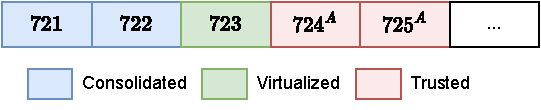
\includegraphics[scale=0.7]{\zkevmdir/figures/architecture/synchronizer/l2-reorganizations-1.drawio}
\caption{Sequencer A.}
\label{fig:l2-reorganizations-1}
\end{figure}

However, let's consider that another sequencer (let's call it sequencer B) closes and sequences a different 724 batch as in the following figure (Figure \ref{fig:l2-reorganizations-2}):
\begin{figure}[H]
\centering
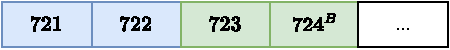
\includegraphics[scale=0.7]{\zkevmdir/figures/architecture/synchronizer/l2-reorganizations-2.drawio}
\caption{Sequencer B.}
\label{fig:l2-reorganizations-2}
\end{figure}

In this case, sequencer A will need to be aware of this situation and re-synchronize its state from $\mathtt{724^B}$. 

To achieve this, \textbf{sequencers} need to check the sequenced transactions present in L1 and re-synchronize their batch flow in case another sequencer virtualizes a different batch. In the zkEVM architecture, there is a component called \textbf{synchronizer} that checks the events produced in L1 when a batch is sequenced so that the sequencer can re-synchronize if needed as in Figure \ref{fig:l2-synchronizer}.

%TODO no se si está be el caption
\begin{figure}[H]
\centering
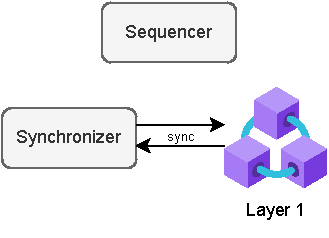
\includegraphics[scale=0.7]{\zkevmdir/figures/architecture/synchronizer/synchronizer-sequencer.drawio}
\caption{The synchronizer looks at Layer 1 and detects instances where a batch has been sequenced but not by the sequencer A. In such cases, it alerts sequencer A to reorganize.}
\label{fig:l2-synchronizer}
\end{figure}


At the moment, reorganizations shouldn't occur in our system due to the presence of a single sequencer, the \textbf{Trusted Sequencer}. The possibility of reorganizations arises only in the event of a back. There's also a slight chance of occurrence during forced batches, where a user is sequencing a batch. However, the design of forced batches is specifically crafted to mitigate such scenarios, a concept we'll explore further in our discussion on forced batches. In general, reorganizations can only occur in the case of a back. If they do happen, they'll exclusively impact the \textbf{Trusted State}, as changes cannot be made to what's written in Layer 1.
%TODO no se que es un back


\section{L1 Reorganizations}
L1 reorganizations happen if there is a reorg in Ethereum itself. In general, L1 reorganizations should never happen because users take for guaranteed that when a state is consolidated, the transaction is done. So, these reorganizations are far more critical, since it might be the case that we have to re-synchronize already virtualized and/or consolidated batches as shown in Fiugre \ref{fig:l1-reorganization}. The \textbf{synchronizer} is also in charge of detecting these situations and inform the \textbf{sequencer} so that the reorg can be performed.

\begin{figure}[H]
\centering
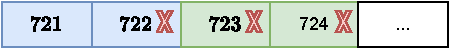
\includegraphics[scale=0.7]{\zkevmdir/figures/architecture/synchronizer/l1-reorganization.drawio}
\caption{A reorganization in L1 requires a change of the state.}
\label{fig:l1-reorganization}
\end{figure}


\section{Synchronizer}
The \textbf{synchronizer} is absolutely necessary to do reorganizations but, in general, also detects and records in the node's \textbf{StateDB} any relevant event from L1 (not only reorgs).